\begin{figure}[htbp]
\centering
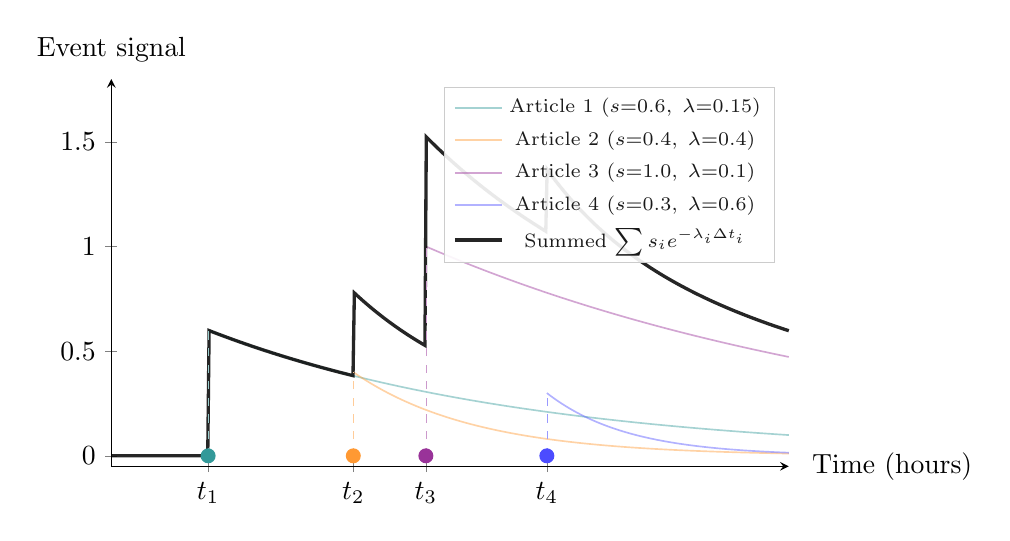
\begin{tikzpicture}
\begin{axis}[
    width=0.84\textwidth,
    height=6.5cm,
    xlabel={Time (hours)},
    ylabel={Event signal},
    xmin=0, xmax=14,
    ymin=-0.05, ymax=1.8,
    xtick={2,5,6.5,9},
    xticklabels={$t_1$, $t_2$, $t_3$, $t_4$},
    ytick={0,0.5,1.0,1.5},
    axis lines=left,
    every axis x label/.style={at={(ticklabel* cs:1.02)}, anchor=west},
    every axis y label/.style={at={(ticklabel* cs:1.02)}, anchor=south},
    legend style={
        at={(0.98,0.98)}, anchor=north east,
        font=\scriptsize, draw=gray!40,
        fill=white, fill opacity=0.9,
        row sep=1pt,
    },
    grid=none,
    clip=false,
]

% --- Individual decay curves (thin, colored) ---
\addplot[domain=2:14, samples=200, teal!70, semithick, opacity=0.5]
    {0.6 * exp(-0.15*(x-2))};
\addlegendentry{Article 1 ($s{=}0.6,\;\lambda{=}0.15$)}

\addplot[domain=5:14, samples=200, orange!70, semithick, opacity=0.5]
    {0.4 * exp(-0.4*(x-5))};
\addlegendentry{Article 2 ($s{=}0.4,\;\lambda{=}0.4$)}

\addplot[domain=6.5:14, samples=200, violet!70, semithick, opacity=0.5]
    {1.0 * exp(-0.1*(x-6.5))};
\addlegendentry{Article 3 ($s{=}1.0,\;\lambda{=}0.1$)}

\addplot[domain=9:14, samples=200, blue!60, semithick, opacity=0.5]
    {0.3 * exp(-0.6*(x-9))};
\addlegendentry{Article 4 ($s{=}0.3,\;\lambda{=}0.6$)}

% --- Summed signal (single expression using boolean conditions) ---
\addplot[domain=0:14, samples=500, black, very thick, opacity=0.85]
    { (x>=2)  * 0.6 * exp(-0.15*(x-2))
    + (x>=5)  * 0.4 * exp(-0.4*(x-5))
    + (x>=6.5)* 1.0 * exp(-0.1*(x-6.5))
    + (x>=9)  * 0.3 * exp(-0.6*(x-9))
    };
\addlegendentry{Summed $\sum s_i e^{-\lambda_i \Delta t_i}$}

% --- Article arrival markers on x-axis ---
\addplot[only marks, mark=*, mark size=2.5pt, teal!80, forget plot] coordinates {(2,0)};
\addplot[only marks, mark=*, mark size=2.5pt, orange!80, forget plot] coordinates {(5,0)};
\addplot[only marks, mark=*, mark size=2.5pt, violet!80, forget plot] coordinates {(6.5,0)};
\addplot[only marks, mark=*, mark size=2.5pt, blue!70, forget plot] coordinates {(9,0)};

% --- Dashed vertical lines at arrivals ---
\draw[teal!40, dashed, very thin] (axis cs:2,0) -- (axis cs:2,0.6);
\draw[orange!40, dashed, very thin] (axis cs:5,0) -- (axis cs:5,0.4);
\draw[violet!40, dashed, very thin] (axis cs:6.5,0) -- (axis cs:6.5,1.0);
\draw[blue!40, dashed, very thin] (axis cs:9,0) -- (axis cs:9,0.3);

\end{axis}
\end{tikzpicture}
\caption{Event signal accumulation. Each article contributes a decaying signal with magnitude $s_k$ and rate $\lambda_k$. The aggregate is the sum of the active article kernels. Curves illustrate the mechanism and are not empirical parameter estimates; the horizontal scale and the displayed rates use hours. The model is inspired by Hawkes-type kernels but does not fit a self-exciting arrival intensity.}
\label{fig:decay_stacking}
\end{figure}
